\graphicspath{ {Figures/technology_stack/} }
\chapter{Τεχνολογίες}\label{ch:Development Stack}
\section{Back-End}
	\subsection{Cloud}
	Μοντέλα υπηρεσιών
		\subsubsection{IaaS}
		\subsubsection{PaaS}
		\subsubsection{SaaS}
		\subsubsection{BaaS}
			Γιατί Parse ?
	Μοντέλα ανάπτυξης
		\subsubsection{Private cloud}
		\subsubsection{Community cloud}
		\subsubsection{Public cloud}
		\subsubsection{Hybrid cloud}
		\subsubsection{NodeJs}
		\subsubsection{Cloud και ασφάλεια Ιατρικών δεδομένων?}
	\subsection{Βάση Δεδομένων}
		\subsubsection{Σχετικά με NoSql}
			NoSql vs Relation DB - βρες κάτι και για medical με nosql. Γιατί NoSql. Γιατί MongoDb.
		\subsubsection{Schema}

\section{Front-End}
	\subsection{Αρχιτεκτονική}
		\subsubsection{MVC αρχιτεκτονικό πρότυπο}\label{sssection:mvc}

		Το σχεδιαστικό μοτίβο Model View Controller (MVC) είναι ένα αρχιτεκτονικό πρότυπο που χρησιμοποιείται στην τεχνολογία λογισμικού και συνήθως στην υλοποίηση web εφαρμογών. Χωρίζει την εφαρμογή σε τρία διασυνδεδεμένα μέρη, με σκοπό τον πλήρη διαχωρισμό της εσωτερικής αναπαράστασης  της πληροφορίας στο σύστημα από τους τρόπους παρουσίασης της πληροφορίας στον χρήστη. Το MVC αποτελείται από τρία στοιχεία: α) Model, β) View, γ) Controller.
		\begin{itemize} 
		\item\textbf{Model:} Το model είναι το κομμάτι της εφαρμογής που αναπαριστά την πληροφορία, δηλαδή τα δεδομένα που χρησιμοποιεί η εφαρμογή και επιβάλλει τις ενέργειες και τους περιορισμούς πάνω σε αυτά.  Στο model τοποθετούμε τις λειτουργίες της εφαρμογής που σχετίζονται με την πρόσβαση στη βάση δεδομένων. Οι λειτουργίες αυτές είναι συναρτήσεις με τις οποίες διαχειριζόμαστε αποτελεσματικά τα δεδομένα που λαμβάνουμε από τη βάση.  Το μοντέλο ανταποκρίνεται σε ερωτήματα από το view καθώς και σε οδηγίες από τον controller για να πραγματοποιήσει ενημερώσεις.
		\item\textbf{View:} Αντιστοιχεί στην γραφική παρουσίαση των δεδομένων του model στο interface του χρήστη. Ο controller, είναι αυτός ο οποίος αποφασίζει πότε θα παρουσιαστούν τα δεδομένα ενώ το view καθορίζει τον τρόπο με τον οποίο θα παρουσιαστούν τα δεδομένα στον χρήστη. Το επίπεδο view θα πρέπει να προσαρμόζεται στις αλλαγές του επιπέδου του model, για αυτό και τα views θα πρέπει να επικεντρώνονται μόνο στην εμφάνιση δεδομένων και να μην εμπλέκονται με την επιχειρηματική λογική του model.
		\item\textbf{Controller:} Ο controller είναι αυτός που παίρνει αποφάσεις, δηλαδή διαχειρίζεται τη σύνδεση των δεδομένων του model με τη λογική του προγράμματος και καθορίζει ποια από τα δεδομένα του model θα παρουσιαστούν από το view στο interface του χρήστη. Ο controller ενημερώνει το view κάθε φορά που αλλάζει το model. Επιπλέον προσθέτει event listeners στο view και ενημερώνει το model όταν ο χρήστης αλληλεπιδρά με το view.
	 \end{itemize}		
	 \begin{figure}[h]
	    \centering
	    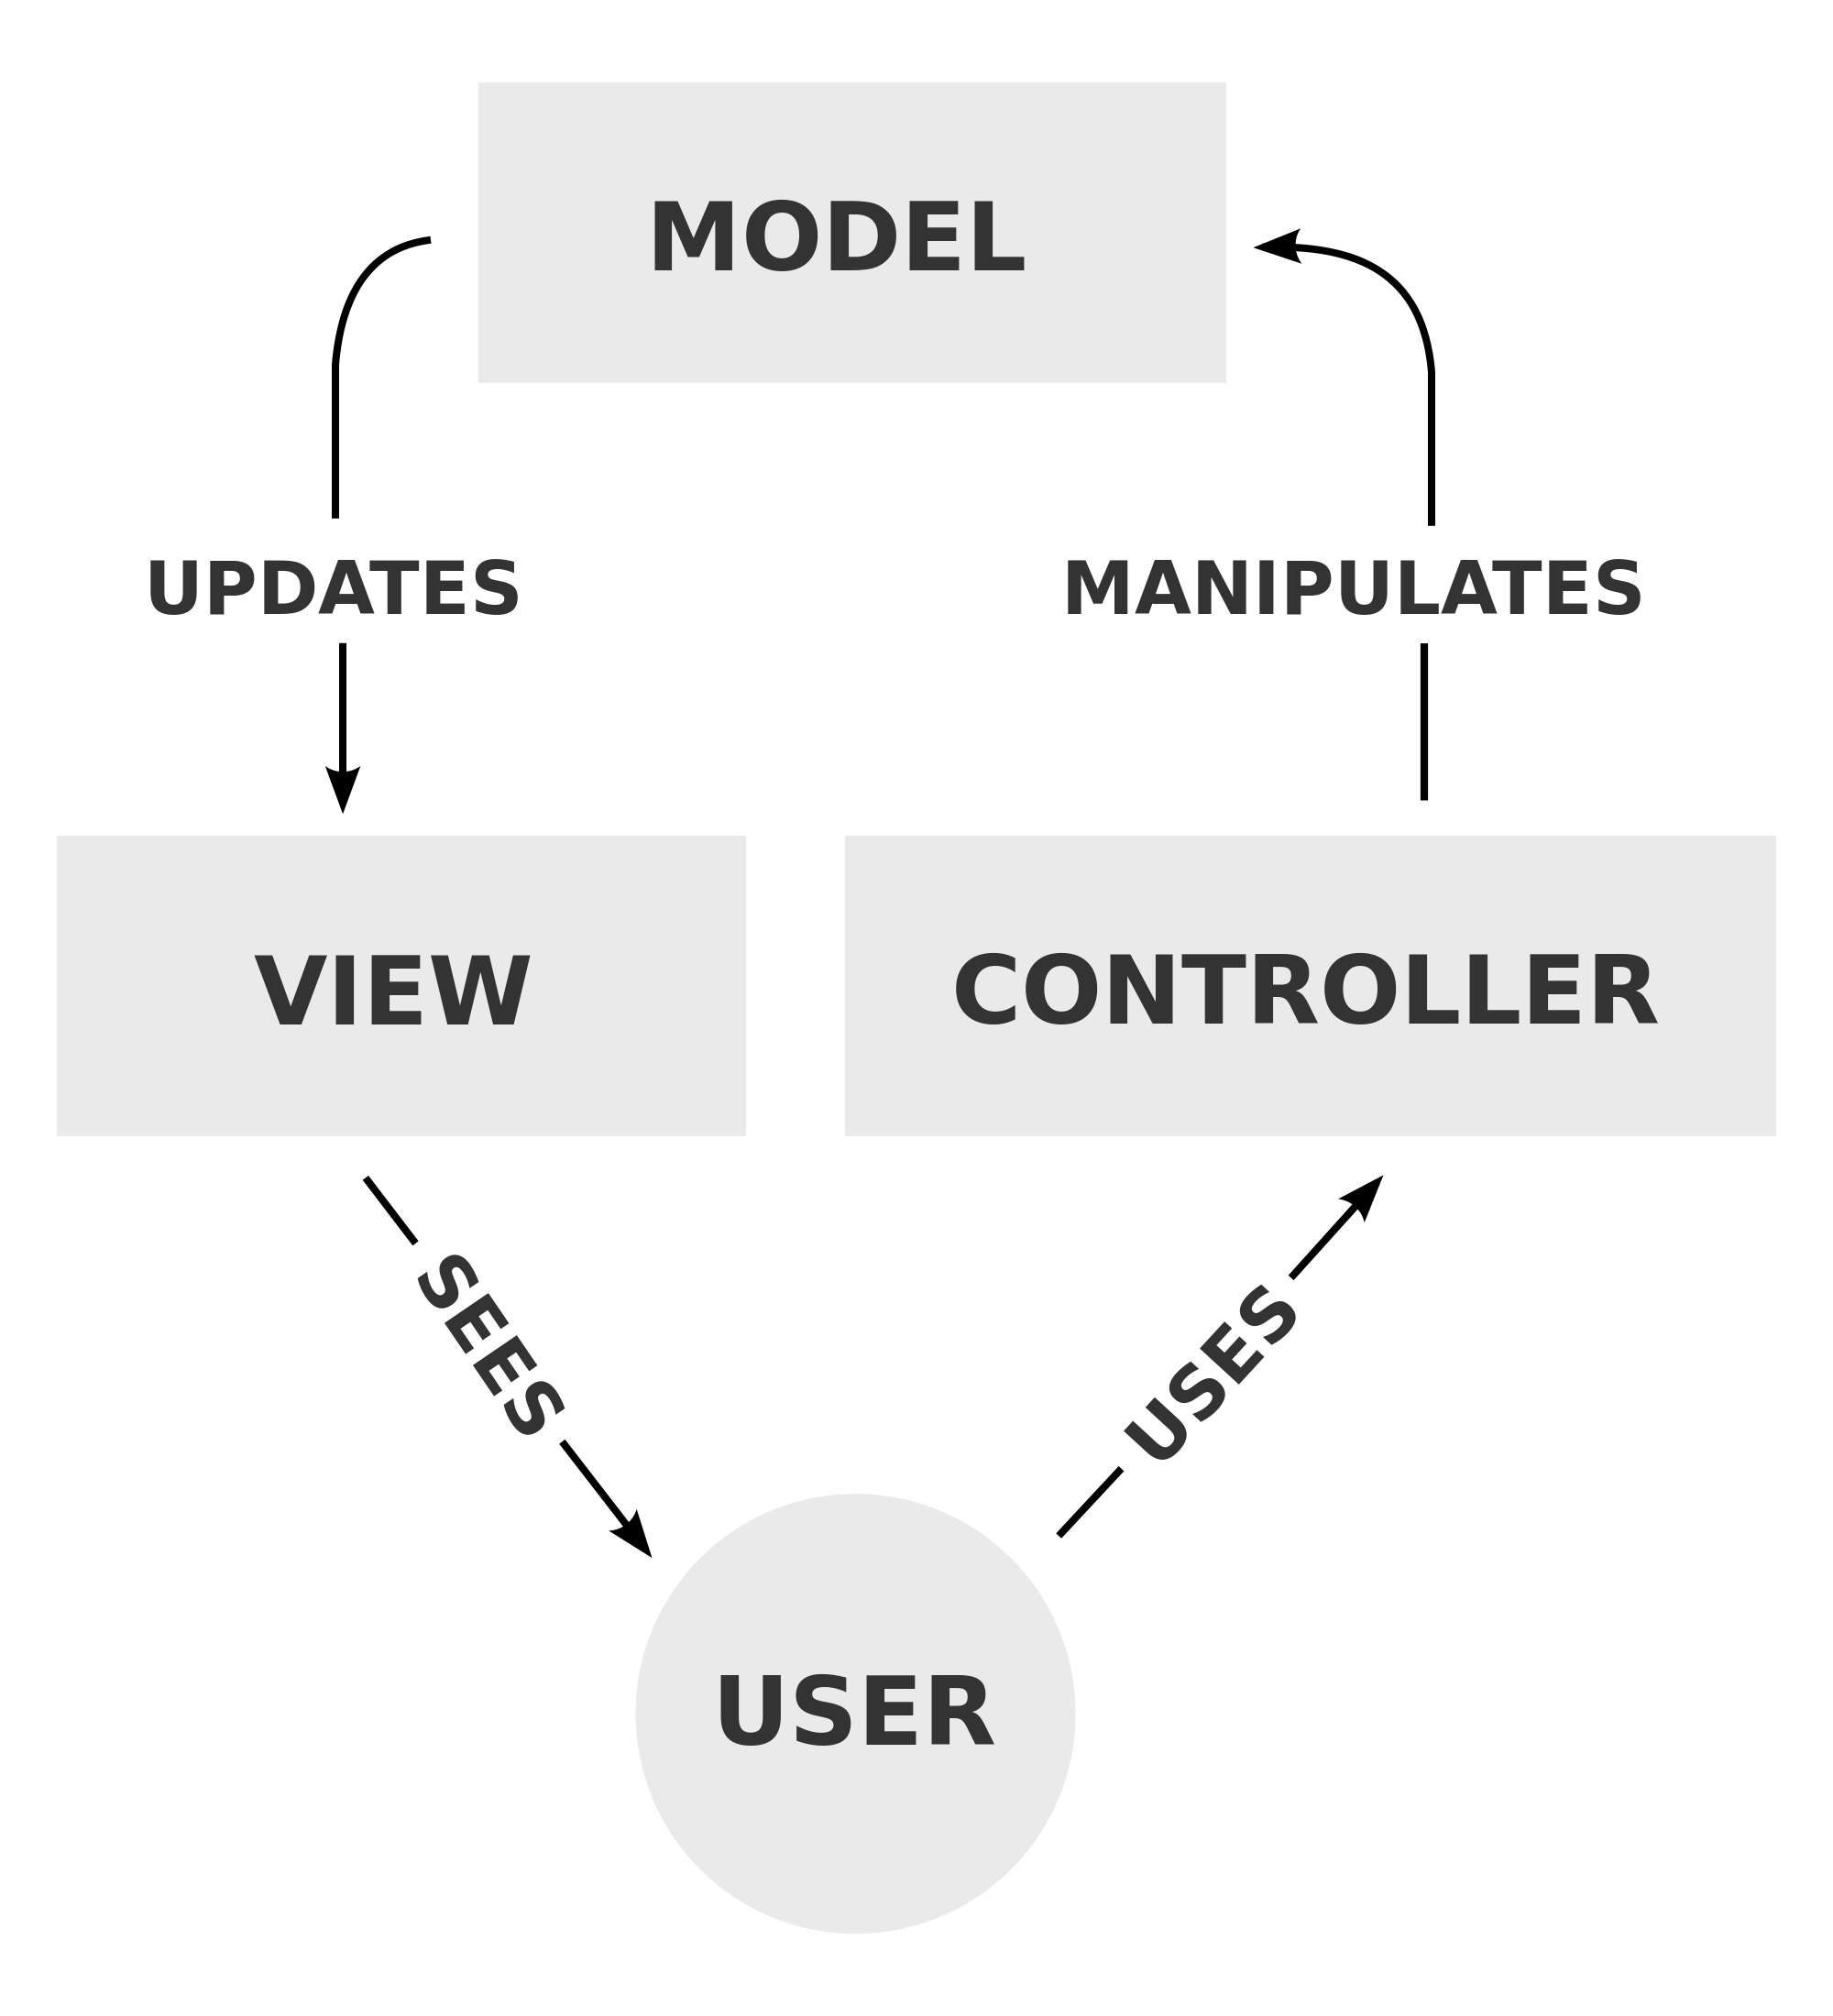
\includegraphics[width=0.7\textwidth]{mvcpattern.png}
	    \caption{Αρχιτεκτονική MVC.}
	    \label{fig:mvc_pattern}
	\end{figure}
		
		
		Η  χρήση της αρχιτεκτονικής MVC κατά την δημιουργία μίας εφαρμογής μας προσφέρει τα εξής βασικά πλεονεκτήματα:
		\begin{itemize}
		\item Διαχωρισμός των προβλημάτων (Separation of Concerns). Ουσιαστικά δημιουργείται μία εφαρμογή η οποία έχει τρία επίπεδα(models, views, controllers) και το κάθε επίπεδο επιτελεί ξεχωριστό έργο και ταυτόχρονα συνεργάζεται με τα άλλα επίπεδα. Στην σωστή υλοποίηση πρέπει τα τρία επίπεδα να είναι πλήρως καθορισμένα και να μην συμπλέκονται. Ο διαχωρισμός αυτός, επιτρέπει την επαναχρησιμοποίηση της επιχειρηματικής λογικής σε διάφορες εφαρμογές και την ανάπτυξη πολλαπλών user interfaces χωρίς να προβληματιζόμαστε από τον κώδικα που διαχειρίζεται την βάση.
		\item \textbf{Επεκτασιμότητα (Scaleability)}. Είναι η δυνατότητα που διαθέτει μία εφαρμογή , να μπορούμε μελλοντικά να προσθέσουμε λειτουργίες σε αυτή ή να αλλάξουμε κάποιες από τις ήδη υπάρχουσες λειτουργίες με σκοπό να επιτύχουμε διαφορετικά αποτελέσματα. 
		\item \textbf{Ελεγξιμότητα (Testability)}. Οι MVC εφαρμογές έχουν την δυνατότητα να είναι πιο εύκολα ελέγξιμες και με τον τρόπο αυτό συντηρούνται πιο εύκολα.  Εφόσον τα συστατικά της αρχιτεκτονικής είναι διακριτά είναι πιο εύκολο να γράφουμε κώδικα που να τεστάρει ξεχωριστά το κάθε κομμάτι, γρήγορα και αποτελεσματικά.
		\item \textbf{Παράλληλη ανάπτυξη από διαφορετικές ομάδες}. Οι προγραμματιστές επιχειρηματικής λογικής  μπορούν να δημιουργούν τις κλάσεις, ενώ οι προγραμματιστές του user interface μπορούν να σχεδιάζουν ταυτόχρονα τις οθόνες. Επίσης μπορούν να γίνονται ενημερώσεις και αλλαγές στο user interface χωρίς να επιβραδύνεται η διαδικασία του business logic.
		\end{itemize}
		
	\subsubsection{MVP αρχιτεκτονικό πρότυπο}
	Το αρχιτεκτονικό πρότυπο Model View Presenter (MVP) αποτελεί ένα παράγωγο αρχιτεκτονικό πρότυπο του MVC \cite{mvpPotel}, το οποίο είναι πολύ δημοφιλές στην ανάπτυξη εφαρμογών για το λειτουργικό σύστημα Android. Στην θεωρία τουλάχιστον, οι εφαρμογές Android είναι στημένες με την λογική του MVC \cite{androidArchAnalysis} όπως περιγράφηκε στην ενότητα \ref{sssection:mvc}, με το Activity ή το Fragment να αποτελεί τον controller και τα xml layouts τα views. Στην πράξη όμως καταλήγει η πλειονότητα του view logic να βρίσκεται στο Activity το οποίο το μετατρέπει σε δομή model-view όπως φαίνεται στο σχήμα \ref{fig:model_view}, κάτι το οποίο σε καμία περίπτωση δεν είναι το επιθυμητό. Στόχος λοιπόν του MVP είναι να λύσει ακριβώς αυτό το πρόβλημα και να πετύχει πλήρη διαχωρισμό μεταξύ του view και του view logic όπως βλέπουμε στο σχήμα \ref{fig:mvp_pattern}.
		
	 \begin{figure}[h]
	    \centering
	    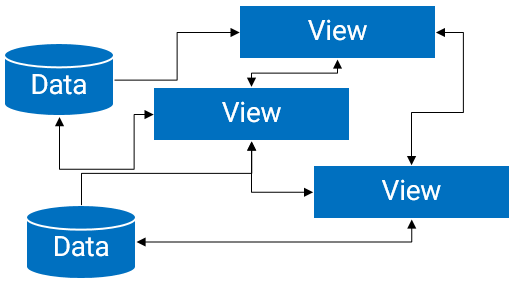
\includegraphics[width=0.7\textwidth]{model_view.png}
	    \caption{Android Model-View αρχιτεκτονικό πρότυπο}
	    \label{fig:model_view}
	\end{figure}
	
	\begin{figure}[h]
	    \centering
	    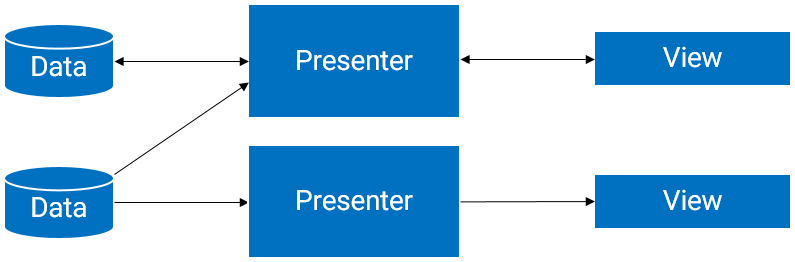
\includegraphics[width=0.7\textwidth]{mvp_pattern.png}
	    \caption{Android MVP αρχιτεκτονικό πρότυπο}
	    \label{fig:mvp_pattern}
	\end{figure}
	
	Πλεονεκτήματα και λόγοι χρήσης του αρχιτεκτονικού προτύπου Model View Presenter\cite{androidHacks}:
	\begin{itemize}
		\item \textbf{Επεκτασιμότητα} η οποία επιτυγχάνεται μέσω του πλήρη διαχωρισμού μεταξύ της εμφάνισης (view) και της λογικής της εμφάνισης (view logic). 
		\item \textbf{Ευκολία Testing} του κάθε στρώματος (layer) της εφαρμογής αφού έχουμε πετύχει σαφή διαχωρισμό μεταξύ τους. Εν γένει η χρήση του μοτίβου MVP προάγει το test driven development της εφαρμογής με όλα τα πλεονεκτήματα που συνεπάγεται η εν λόγω τεχνική ανάπτυξης.
	\end{itemize}
	
	Το αρχιτεκτονικό πρότυπο MVP όπως δηλώνει και το όνομα του αποτελείται από τα παρακάτω τρία στοιχεία α) Model β) View γ) Presenter :
	\begin{itemize}
		\item \textbf{Model: } Το model στο αρχιτεκτονικό πρότυπο MVP επιτελεί της ίδιες λειτουργίες με αυτές στο MVC όπως περιγράφηκαν παραπάνω στην ενότητα \ref{sssection:mvc}.
		\item \textbf{View: } Το view υλοποιείται συνήθως μέσω κάποιου Activity ή Fragment (εξαρτάται από την συγκεκριμένη αρχιτεκτονική της εφαρμογής), και περιέχει αναφορά στον presenter ο οποίος το χειρίζεται. H εν λόγω αναφορά πραγματοποιείται με χρήση του σχεδιαστικού μοτίβου dependency injection και ιδανικά με χρήση του Dagger. Κάθε φορά που ο χρήστης αλληλεπιδρά με κάποια λειτουργία (π.χ κουμπί) του view, καλείται η αντίστοιχη συνάρτηση του presenter ο οποίος επικοινωνεί με το model και λέει εν τέλει στο view τι θα εμφανίσει.
		\item \textbf{Presenter: } Ο Presenter είναι λειτουργεί ως το ενδιάμεσο στάδιο - ενορχηστρωτής μεταξύ του view και του model. Είναι υπεύθυνος για την απόκτηση των δεδομένων από το model και την παρουσίαση τους στο view, αλλά σε αντίθεση με την κλασσική αρχιτεκτονική MVC είναι υπεύθυνος για τις αλλαγές που γίνονται στο view όταν ο χρήστης αλληλεπιδρά μαζί του.
	\end{itemize}
	
	Για να αποσαφηνιστεί πλήρως η λειτουργία του και να γίνει πιο εύκολα κατανοητό στο σχήμα \ref{fig:mvp_workflow} βλέπουμε ένα χαρακτηριστικό παράδειγμα.
	
	\begin{figure}[h]
	    \centering
	    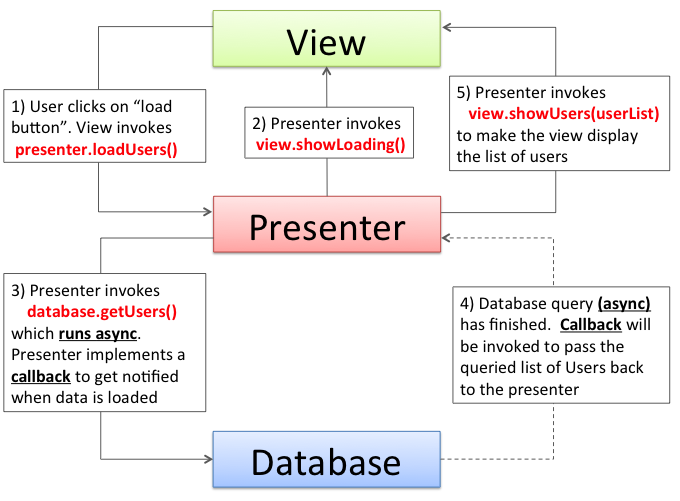
\includegraphics[width=0.7\textwidth]{mvp_workflow.png}
	    \caption{Παράδειγμα MVP σε Android}
	    \label{fig:mvp_workflow}
	\end{figure}

	\subsection{Frameworks}
	
		Το framework, στον προγραμματισμό ηλεκτρονικών υπολογιστών, είναι μια αφηρημένη έννοια με την οποία κοινός κώδικας ο οποίος παρέχει γενικές λειτουργίες, μπορεί να επανεγγραφεί επιλεκτικά ή να εξειδικευτεί μέσω του κώδικα κάποιου χρήστη ώστε να χρησιμοποιηθεί για συγκεκριμένες λειτουργίες. Τα frameworks είναι μια ειδική περίπτωση βιβλιοθηκών λογισμικού που εμπεριέχουν επαναχρησιμοποιήσιμα κομμάτια κώδικα σε μια καλά καθορισμένη διεπαφή προγραμματισμού εφαρμογών (API), που όμως περιέχουν κάποια βασικά χαρακτηριστικά γνωρίσματα που τα διαφοροποιούν από τις κανονικές βιβλιοθήκες. Κάποια από τα γνωρίσματα αυτά είναι: αντιστροφή του ελέγχου (η ροή του προγράμματος υπαγορεύεται από το framework και όχι από αυτόν που το χρησιμοποιεί), προκαθορισμένη συμπεριφορά, επεκτασιμότητα (μπορεί να επεκταθεί από το χρήστη συνήθως με επανεγγραφή  ή εξειδίκευση του κώδικα ώστε να εκτελούνται συγκεκριμένες λειτουργίες. \cite{Framework}

	
		\subsubsection{Express Framework}

		Το Express.js είναι ένα framework του Node.js, σχεδιασμένο για να χτίζει μίας σελίδας, πολλών σελίδων, και hybrid web εφαρμογές. Είναι το προκαθορισμένο framework που χρησιμοποιείται πάνω στο node.js.  Ο δημιουργός του TJ Holowaychuck το περιέγραψε ως ένα "Sinatra inspired server", πράγμα που σημαίνει ότι είναι σχετικά ελάχιστο, με πολλά χαρακτηριστικά διαθέσιμα ως πρόσθετα. Το express είναι το backend της στοίβας MEAN.
		
		\subsubsection{Angular}
		Το AngularJS είναι ένα από τα πιο δημοφιλή ανοιχτού κώδικα JavaScript framework που χρησιμοποιείται για την κατασκευή και τη δομή σύγχρονων διαδικτυακών εφαρμογών, κυρίως εφαρμογών μίας σελίδας. Αναπτύχθηκε από την Google και από μία κοινότητα προγραμματιστών για την αντιμετώπιση των πολλών προκλήσεων που ανέκυψαν κατά την ανάπτυξη των εφαρμογών μίας σελίδας.  Στόχος του είναι να απλοποιήσει τόσο την ανάπτυξη όσο και το testing αυτών των εφαρμογών, παρέχοντας ένα framework για client-side model-View-Controller (MVC) και το model-view-viewmodel (MVVM) αρχιτεκτονικές, μαζί με τα συστατικά που χρησιμοποιούνται συνήθως στις εφαρμογές Διαδικτύου.
	   \\
			    \textbf{Αρχιτεκτονική}
	 \\	
		Κατά την εκκίνηση της εφαρμογής, το πρόγραμμα περιήγησης φορτώνει το HTML αρχείο και το παρσάρει στο DOM αρχείο, και μαζί με αυτό στο angular.js script. Μόλις το DOM αρχείο έχει φορτωθεί, το AngularJS αναζητά την εντολή ng-app η οποία ορίζει τα όρια της εφαρμογής. Εάν ορίζεται κάποιο module μέσα στην οδηγία, τότε χρησιμοποιείται για να ρυθμιστεί το \$injector, που δημιουργεί τo \$compile service καθώς και το \$ rootScope. Τότε μεταγλωττίζεται το DOM και συνδέεται στο \$ rootScope μετά από το οποίο εκτελούνται οι υπόλοιπες εντολές (αν υπάρχουν). Στο σχήμα \ref{fig:angularjs} φαίνεται ο κύκλος εκκίνησης του AngularJS.
	  \begin{figure}[h]
	    \centering
	    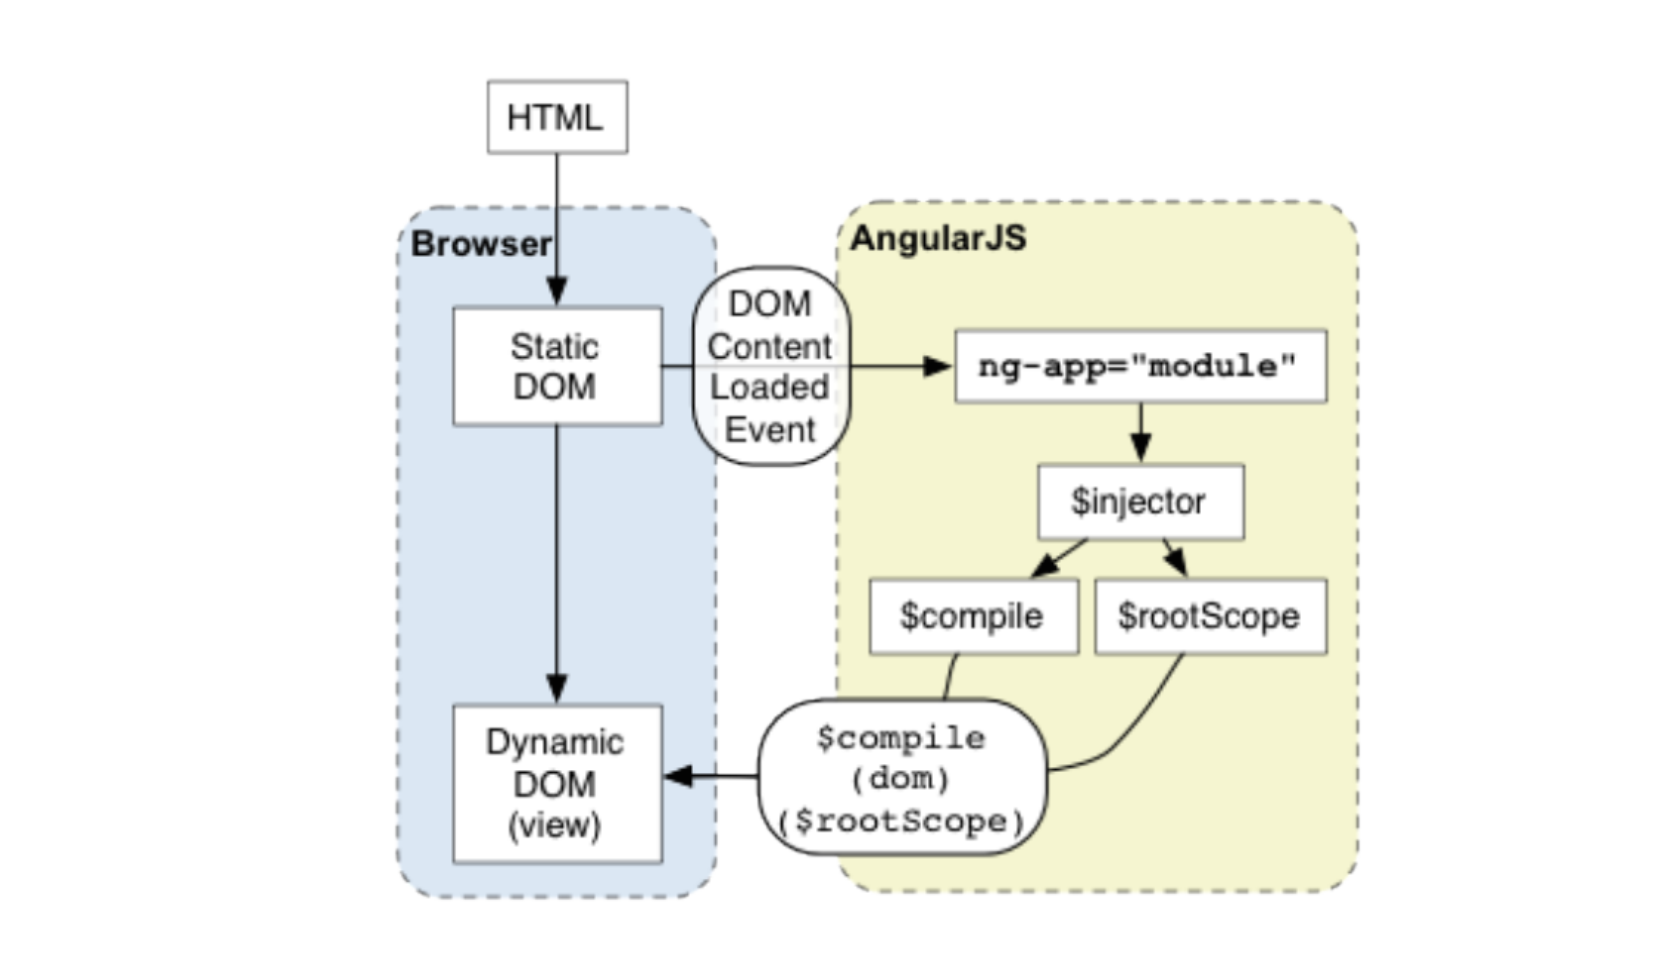
\includegraphics[width=0.7\textwidth]{angularjs.png}
	    \caption{AngularJS κύκλος εκκίνησης.}
	    \label{fig:angularjs}
	\end{figure}

	Κάποια από τα βασικά χαρακτηριστικά του AngularJS είναι:
	\begin{itemize}
	\item Two Way Data-binding. Αυτό πρακτικά σημαίνει ότι όταν αλλάζει το model αλλάζει και το view, και όταν αλλάζει το  view αλλάζει και το model.  Το Two Way Data-binding εξηγείται καλύτερα με ένα παράδειγμα: 
	
	
	\lstinputlisting[language=Html]{two_way_data_binding.html}

	Αν ο χρήστης αλλάζει κάποια τιμή του model μέσω εισόδου στο view, τότε το AngularJs αποθηκεύει την τιμή
αυτή σε μια μεταβλητή. Το στοιχείο h1 στην συνέχεια ενημερώνεται αυτόματα ώστε να αντικατοπτρίζονται οι αλλαγές στην τιμή της μεταβλητής του model. Το view ενημερώνεται ακόμα και αν η μεταβλητή αλλάξει χειροκίνητα με χρήση JavaScript.\cite{angular}

	\item  HTML Templates. Ενώ άλλα JavaScript frameworks χρησιμοποιούν ένα template system που βασίζεται στην HTML με ειδική σήμανση το οποίο μπορεί να είναι δυσκολεύει τους προγραμματιστές, το AngularJS δεν στηρίζεται σε εξωτερικές template engines αλλά χρησιμοποιεί ένα templating σύστημα, που είναι χτισμένη πάνω στην HTML με έξυπνη χρήση των ng- χαρακτηριστικών. Το πρόγραμμα περιήγησης διαβάζει την HTML και "ψάχνει"  ng - directives τα οποία, όταν εκτελεστεί, δεσμεύουν το view στο model.

    \item Dependency Injection. Το dependency injection ενθαρρύνεται πολύ από το AngularJS και είναι ένα από τα συστατικά του, που βελτιώνει σε μεγάλο βαθμό το testability του. Το dependency injection είναι ένα design pattern λογισμικού στο οποίο σε ένα αντικείμενο ορίζονται οι εξαρτήσεις του και δεν τις δημιουργεί μόνο του. Πρόκειται ουσιαστικά για την αφαίρεση των hard-coded εξαρτήσεων κάνοντας δυνατό να αλλάξουν οι εξαρτήσεις όποτε χρειαστεί.
      Ένα παράδειγμα είναι όταν έχεις μία συνάρτηση η οποία παίρνει μία παράμετρο, όπως το ακόλουθο παράδειγμα:
    	
	\lstinputlisting[language=JavaScript]{angular_dependency_injection.js}

Το παραπάνω παράδειγμα είναι εύκολο να το τεστάρουμε, επειδή το στοιχείο που εισάγεται στην συνάρτηση μπορεί να είναι είτε ένα πραγματικό αντικείμενο ή ένα αντικείμενο για τους σκοπούς των τεστ. Ο διαχωρισμός σε μικρότερα πιο εύκολα ελέγξιμα συστατικά μπορεί να βοηθήσει πολύ στην ανίχνευση των σφαλμάτων.

    \item Deep Linking. Σε μια εφαρμογή μίας σελίδας είναι σημαντικό να διατηρείται η κατάσταση της εφαρμογής στο url, έτσι ώστε οι χρήστες είναι σε θέση να βάλουν κάποιο σελιδοδείκτη ή να μοιραστούν κάποιον σύνδεσμο σε διάφορες καταστάσεις της εφαρμογής.Το AngularJS χρησιμοποιεί το HTML5 history API  μαζί με ένα (\#!) εφεδρικό για παλαιότερα προγράμματα περιήγησης. Η λειτουργία αυτή είναι εξαιρετικά ισχυρή στη σύγχρονη εποχή των κοινωνικών δικτύων και του sharing.

	\item Directives. Τα directives είναι κάτι μοναδικό στο AngularJS και επιτρέπουν την επέκταση της λειτουργικότητας της HTML. Ενώ το AngularJS έχει μια συλλογή από προκαθορισμένα directives, μπορεί να επεκταθεί με συγκεκριμένες λειτουργικότητες σε σημείο που να επιτρέπει στον χρήστη να δημιουργήσει το δικό του DSL (Domain specific language). Επίσης επιτρέπει να δημιουργηθούν προσαρμοσμένα στοιχεία DOM, καθώς και χαρακτηριστικά και κλάσεις στα οποία μπορούν να προστεθούν λειτουργικότητες. Το επόμενο παράδειγμα από το επίσημο documentation του AngularJS δείχνει ότι για παράδειγμα γίνεται να επιτραπούν data-bindings για ένα html στοιχείο, αν υπάρχει ένα συγκεκριμένο χαρακτηριστικό. \cite{angular-directives}
\\*
\textbf{HTML:}

	\lstinputlisting[language=Html]{angular_directives.html}
 
\textbf{JavaScript:}

	\lstinputlisting[language=JavaScript]{angular_directives.js}


	\item \$http service. Το AngularJS είναι εξαιρετικά ευέλικτο στον τρόπο που επικοινωνεί με τα διαφορετικά backends. Αντί να βασίζεται αποκλειστικά στο REST interface, επικοινωνεί ελεύθερα μέσω των XMLHttpRequests του προγράμματος περιήγησης ή μέσω του JSONP. Παρόλο που το \$ http service προσθέτει http headers ως προεπιλογή στα αιτήματα του,  είναι εύκολα διαμορφώσιμα μέσω του \$httpProvider.defaults.headers.
	\end{itemize}


		\subsubsection{JQuery}

		\subsubsection{Bootstrap}
	Το bootstrap είναι ένα πάρα πολύ δυνατό front-end framework για την ταχύτερη και ευκολότερη ανάπτυξη ιστοσελίδων. Είναι μία συλλογή εργαλείων ανοιχτού κώδικα και περιλαμβάνει HTML και βασισμένα στο CSS πρότυπα σχεδιασμού για κοινά στοιχεία διεπαφής χρήστη, όπως τυπογραφίας, φόρμες, κουμπιά, πίνακες, dropdowns, alerts, μπάρες, και πολλά άλλα, καθώς και προαιρετικές επεκτάσεις JavaScript.Το bootstrap είναι συμβατό με όλες τις τελευταίες εκδόσεις των προγραμμάτων πλοήγησης και υποστηρίζει "responsive web design". Αυτό σημαίνει πως η διάταξη των ιστοσελίδων προσαρμόζεται δυναμικά, λαμβάνοντας υπόψιν τα χαρακτηριστικά της συσκευής που το χρησιμοποιεί (σταθερός υπολογιστής, κινητό, τάμπλετ κλπ.). 
	
	Το bootstrap είναι modular και αποτελείται από μικρότερα LESS stylesheets τα οποία υλοποιούν τα διάφορα στοιχεία του πακέτου εργαλείων. Ένα stylesheet, με όνομα bootstrap.less περιλαμβάνει τα επιμέρους stylesheets. Οι προγραμματιστές μπορούν να προσαρμόσουν και οι ίδιοι το bootstrap, καθώς τους δίνεται η δυνατότητα να επιλέξουν τα στοιχεία που θέλουν να χρησιμοποιήσουν. Αναπροσαρμογές γίνονται σε περιορισμένο όμως βαθμό, μέσω ενός κεντρικού stylesheet. Πιο ουσιαστικές αλλαγές πραγματοποιούνται με LESS δηλώσεις. Η χρήση των LESS stylesheets επιτρέπει τη χρήση μεταβλητών, συναρτήσεων καθώς και mixins. Επιπλέον, ο σχεδιαστής μπορεί να επιλέγει σε μια φόρμα τα επιθυμητά στοιχεία και να τα προσαρμόζει, σε τιμές διαφόρων εναλλακτικών λύσεων για τις ανάγκες του. Στη συνέχεια δημιουργείται ένα πακέτο που περιλαμβάνει ήδη το προ-χτισμένο CSS stylesheet.
	
	Το bootstrap παρέχει ένα σύνολο από stylesheets που παρέχουν βασικούς ορισμούς στυλ για όλα τα βασικά HTML στοιχεία με. Αυτά παρέχουν ενιαία, σύγχρονη εμφάνιση για πίνακες, μορφοποίηση κειμένου, καθώς και για τα στοιχεία μιας φόρμας. Επιπλέον των HTML στοιχείων, το bootstrap περιέχει και άλλα στοιχεία περιβάλλοντος τα οποία χρησιμοποιούνται συχνά. Αυτά περιλαμβάνουν κουμπιά με προηγμένα χαρακτηριστικά ( π.χ. ομαδοποίηση κουμπιών ή drop-down επιλογή, οριζόντιες και κάθετες καρτέλες, σελιδοποίηση, κ.λ.π. ), ετικέτες, προηγμένες τυπογραφικές δυνατότητες, εικονίδια, προειδοποιητικά μηνύματα και μια γραμμή προόδου. Τέλος, το bootstrap περιέχει πολλά συστατικά JavaScript σε μια μορφή jQuery plugin. Παρέχουν πρόσθετα στοιχεία διεπαφής χρήστη όπως παράθυρα διαλόγου, επεξηγήσεις, και καρουσέλ. Μπορούν επίσης να επεκτείνουν τη λειτουργικότητα ορισμένων υφιστάμενων στοιχείων της διασύνδεσης, όπως για παράδειγμα μια αυτόματη πλήρη λειτουργία για πεδία εισαγωγής.

		
	\subsection{Express και Jade Template Engine}
	\subsection{Mockups}
	\subsection{Διασύνδεση με Social Networks}

\section{Mobile}
	\subsection{Mobile OS}
		Ανάλυση διαθέσιμων OS (Android, iOS, Windows)
	\subsection{Android}
		Υλοποίηση με Android, γιατί;
		Material design ? Αν δεν είναι API Level 21?
	\subsection{Mockups}
	\subsection{Διασύνδεση με Social Networks}
